\chapter[Introduction]{\uline{Introduction}}
\section[Fin design parameters]{\uline{Fin design parameters:}}

\hspace{0.2 cm} We consider the problem of designing a thermal fin to effectively remove heat from a surface. The two-dimensional fin, shown in Figure 1, consists of a vertical central post and four horizontal subfins; the fin conducts heat from a prescribed uniform flux source at the root, $\gamma_{root}$ , through the large-surface-area subfins to surrounding flowing air. The fin is characterized by a five-component parameter vector, or input, $\mu = (\mu_1 , \mu_2 , . . . , \mu_5 )$,where $\mu_i = k^i , i = 1, . . . , 4,$ and
$\mu_5 = Bi$; μ may take on any value in a specified design set $D \in R^5$ .

\begin{figure}[h!]
	\centering 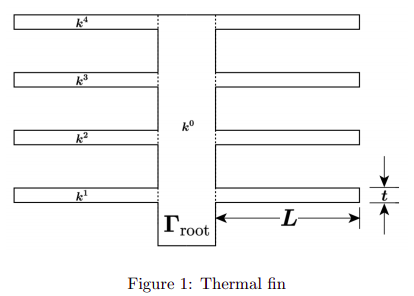
\includegraphics[scale=0.5]{Images_Fichiers/fin.png}
%\legend{template}
%\label{1CCG}
\end{figure}

Here $k^i$ is the thermal conductivity of the ith subfin (normalized relative to the post conductivity $k^0 ≡ 1$); and Bi is the Biot number, a nondimensional heat transfer coefficient reflecting convective transport to the air at the fin surfaces (larger Bi means better heat transfer). For example, suppose we choose a thermal fin with $k^1 = 0.4, k^2 = 0.6, k^3 = 0.8, k^4 = 1.2, and Bi = 0.1$; for this particular configuration $\mu = {0.4, 0.6, 0.8, 1.2, 0.1}$, which corresponds to a single point in the set of all possible configurations D (the parameter or design set).The post is of width unity and height four; the subfins are of fixed thickness t = 0.25 and length L = 2.5.


\section[Governing equation]{\uline{Governing equation:}}

\hspace{0.2 cm} We are interested in the design of this thermal fin, and we thus need to look at certain outputs or cost-functionals of the temperature as a function of $\mu$. We choose for our output $T_{root}$ , the average steady-state temperature of the fin root normalized by the prescribed heat flux into the fin root. The particular output chosen relates directly to the cooling efficiency of the fin lower values of $T_{root}$ imply better thermal performance. The steadystate temperature distribution within the fin, $u(\mu)$, is governed by the elliptic partial differential equation:

\equaframe{ -k^i \Delta u^i = 0 \quad in \quad \Omega^i , i = 0, . . . , 4,}{(1)}

where $\Delta$ is the Laplacian operator, and $u^i$ refers to the restriction of u to $\Omega^i$. Here $\Omega^i$ is the region of the fin with conductivity $k^i$ , i = 0, . . . , 4 : $\Omega^i$ is thus the central post, and $\Omega^i$, i = 1, . . . , 4, corresponds to the four subfins. The entire fin domain is denoted $\Omega(\bar{\Omega}= \cup_{i=0}^4 \bar{\Omega}^i )$.


\section[Boundary conditions]{\uline{Boundary conditions:}}

\hspace{0.2 cm} The boundary $\Omega$ is denoted $\Gamma$. We must also ensure \uline {continuity of temperature and heat flux} at the conductivity discontinuity interfaces $\Gamma_{int}^i$ = $\partial\Omega^0$ $\cap$ $\partial\Omega^i$, i = 1, . . . , 4, where $\partial\Omega^i$ denotes the boundary of $\Omega^i$. We have on $\Gamma_{int}^i$ i = 1, . . . , 4 :
\begin{gather*}
  \equaframe{ u^0 = u^i }{(2)}
\\ 
  \equaframe{-(\Delta u^0 . n^i) = −k^i (\Delta u^i . n^i)}{(3)}
\end{gather*}
Here $n^i$ is the outward normal on $\partial\Omega^i$ . 
Finally, we introduce a \uline{Neumann flux boundary condition on the fin root}:
\equaframe{-(\Delta u^0 . n^0) = −1 \quad on \quad  \Gamma_{root}}{(4)}
which models the heat source; and \uline{a Robin boundary condition}:
\equaframe{-k^i(\Delta u^i . n^i) = −Bi u^i \quad on \quad \Gamma_{ext}^i  i = 0, . . . , 4 }{(5)}

which models the convective heat losses. Here Γ iext is that part of the boundary of $\Omega^i$ exposed to the flowing fluid; note that $\cap_{i=0}^4 \Gamma_{ext}^i=\Gamma /\Gamma_{root}$. The average temperature at the root, $\Gamma_{root}(\mu)$, can then be expressed as $l^O(u(\mu))$,where:
\equaframe{l^O(v) = \int_{\Gamma_{root}}v }{(6)}

(recall $\Gamma_{root}$ is of length unity). Note that $l(v)=l^O(v)$ for this problem.








































